\documentclass{article}

\XeTeXdefaultencoding utf-8

\usepackage{fontspec}	% An automatic interface to feature-rich fonts
\usepackage{xunicode}	% Generate Unicode characters from accented glyphs
\usepackage{xltxtra}	% "Extras" for LaTeX users of XeTeX

% Flexible and complete interface to document dimensions
% \usepackage{geometry}
% \geometry{a4paper}

\usepackage{graphicx}

\usepackage[colorlinks]{hyperref}

% \usepackage[francais]{babel} % Multilingual support for Plain TeX or LaTeX

\defaultfontfeatures{Mapping=tex-text}

%%%%%%%%%%%%%%%%%%%%%
% Fonts in document %
%%%%%%%%%%%%%%%%%%%%%

% Use open fonts
% --------------

 \setmainfont{Linux Libertine}
 \setsansfont{Andika Basic}
 \setmonofont{Inconsolata}

% Use Microsoft fonts
% -------------------

% \setmainfont{Constantia}
% \setsansfont{Corbel}
% \setmonofont{Consolas}

\usepackage{color}
\definecolor{NoteBackground}{rgb}{0.96,0.97,0.98}
\definecolor{NoteFrame}{rgb}{0.5,0.5,0.5}
\makeatletter\newenvironment{note}{%
   \noindent \begin{lrbox}{\@tempboxa}\begin{minipage}{\columnwidth}\textbf{Note:}}{\end{minipage}\end{lrbox}%
   \fcolorbox{NoteFrame}{NoteBackground}{\usebox{\@tempboxa}}
}\makeatother

\newcommand{\internal}{\textsl{internal}~}

\title{UCard SDK}
\author{IL4P}

\begin{document}

\maketitle

\tableofcontents

\section{Introduction}

\emph{UCard} for \emph{Universal Card}

versatile usage

set of tools on top of \emph{libfreefare} \cite{libfreefare}

simple API

NOT all-in-one

NOT designed with genericity

DESFire
DESFireUCard
TransportCard
AccessCard

API Provides:
  - On card operations
	- Off card operations

API for:
  - Card manipulation API
	- Kiosk API

\section{Key Features}

\begin{itemize}
  \item Easy to use high level API;
	\item Based on cheap and ubiquitous Mifare DESFire cards;
	\item No knowledge of Mifare DESFire internals required;
  \item Full read-only access to the card owner.
\end{itemize}

\section{Installing the SDK}

PC/SC-lite

libusb

libnfc \cite{libnfc}

libfreefare \cite{libfreefare}

libucard

Building the Examples

\section{Using the SDK}

\subsection{Cards Initial Personalisation}

Before it can be used as a \emph{UCard} target, a \emph{Mifare
DESFire} target has to programmed so that it contains a minimal set of
information.  This operation has to be performed once, when the card is
issued to the customer.

% TODO Is it reversible ?

The initialisation routine will create an application on the card that
stores the following pieces of information:

\begin{enumerate}
  \item The UCard version;
	\item The UCard owner's full name;
\end{enumerate}

Each time a card is presented to a NFC coupler, the libucard will look
for such an application and use the version information to determine
	the capabilities of the card.

\begin{figure}[htp]
  \centering
  \includegraphics[scale=1]{intitial-personalisation}
\end{figure}

\subsection{Card Protection}

CreateApplication / DeleteApplication / ListApplication may be free or
password-protected with the card owner PIN.

%Application
%  File 0 - meta (file1=# tickets 1h, file-2=#tickets 24h,	file-3=travel record)em
%	File 1 - 

\subsection{Applications Versioning}

The master key of an application stores the application version.
When an UCard target is selected by the coupler, the application
version on card is checked to detect any possible update.

\section{Modules}

\subsection{Credit/Debit}

The security mechanism for \emph{Value Files} is dramatically
different from the one available for other file types: an
authentication with the \emph{Read \& Write Key} (and only this key)
is required for using the \texttt{ucard\_value\_file\_credit()}, while
an authentication with \textbf{any} key is nought to use all other
functions.

\section{Card Applications}

% FIXME: Should be generated from the XSD file (stylesheets/ucard.xsd).

It's an XML file

\begin{figure}[htp]
  \centering
  \includegraphics[width=\textwidth]{code-generation}
\end{figure}

Namespace \texttt{http://il4p.fr/TR/UCard}

applications

application
\begin{description}
	\item[name] Application name in a computer-friendly form (e.g.
	\emph{my\_application});
	\item[aid] Application IDentifier in hexadecimal (e.g. \emph{0x123456}).
\end{description}

\subsection{Keys}

keys

key
\begin{description}
	\item[name] Key name in a computer-friendly form (e.g.
	\emph{master-key});
	\item[type] Key type (e.g. \emph{3DES});
	\item[data] Key data (e.g. \emph{0x0000000000000000}).
\end{description}


\begin{note}
In order to ease generation of many random keys, the SDK provide an
utility called \textbf{ucard-keygen} which can be found in the
\texttt{tools/ucard-keygen} directory.
\end{note}

\subsection{Files}

\section{Kiosk Applications}

In the UCard terminology, a \emph{kiosk} is a system with at least one
NFC coupler acting as a NFC initiator, and a control software named a
\emph{kiosk application}.

The \texttt{libucard(4)} library provides a convenient API to build
kiosk applications in an efficient and error-prone way.

\begin{figure}[hp]
	\centering
  \includegraphics{kiosk-001}
\end{figure}

A \emph{kiosk} has first to be created using the
\texttt{kiosk\_new()} function.  Before using the kiosk, it has to be
configured using the \texttt{kiosk\_setup()} function, and at least
one NFC initiator should be associated with it. This is achieved using
either the \texttt{kiosk\_add\_device()} function, or the
\texttt{kiosk\_devices\_scan()} function in which case the kiosk
application will use all NFC devices available on the system.

When \texttt{kiosk\_start()} is called, the library will start one
thread per NFC initiator which will look for an UCard on a regular
basis.

The \texttt{kiosk\_wait()} function can be used to block the calling
thread until a card has been presented to a NFC initiator or a timeout
occurs.

The \texttt{kiosk\_stop()} function will unconditionally terminate all
threads.


\begin{figure}[hp]
	\centering
  \includegraphics{kiosk-002}
\end{figure}


\section{API Reference}

\begin{figure}[htp]
  \centering
  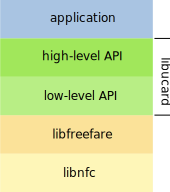
\includegraphics[scale=1]{layers}
	\caption{An UCard application software stack.}
\end{figure}

\begin{figure}[htp]
  \centering
  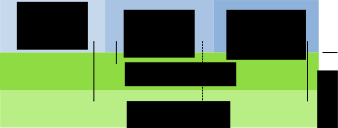
\includegraphics[scale=1]{applications}
	\caption{Applications can use both the low-level and high-level APIs.}
\end{figure}



\subsection{Card Manipulation API}

% ------ CARD CREATION FUNCTIONS

\texttt{ucard\_initialise()}

\texttt{ucard\_personalise()}

% ------

\internal \texttt{ucard\_application\_create()}

% ------ CARD OWNER FUNCTIONS

\texttt{ucard\_application\_delete()}

\texttt{ucard\_change\_master\_key()}

\texttt{ucard\_explain()}

% ------ CARD SHOP FUNCTIONS

\texttt{ucard\_value\_get()}

\texttt{ucard\_value\_credit()}

\texttt{ucard\_value\_debit()}

\texttt{ucard\_value\_limited\_credit()}

\texttt{ucard\_record\_write()}

\texttt{ucard\_record\_read()}

\texttt{ucard\_record\_clear()}

\texttt{ucard\_data\_read()}

\texttt{ucard\_data\_write()}

\texttt{ucard\_transaction\_commit()}

\texttt{ucard\_transaction\_abort()}

\texttt{ucard\_transaction\_start()}

\subsection{Kiosk API}

\texttt{kiosk\_setup()}

\texttt{kiosk\_wait\_ucard()}

\texttt{ucard\_application\_select()}

\texttt{ucard\_application\_update()} INTERNAL

% ---- OTHER FUNCTIONS

\texttt{<vendor>\_<file>\_<action>()}

Available actions depends on the \texttt{file} type.

\subsubsection{Value files actions}

\texttt{<vendor>\_<file>\_credit()}

\texttt{<vendor>\_<file>\_debit()}

\subsubsection{OTP file actions}

\texttt{<vendor>\_<file>\_append()}

\texttt{<vendor>\_<file>\_read()}

\subsubsection{RAW data actions}

\texttt{<vendor>\_<file>\_read()}

\texttt{<vendor>\_<file>\_write()}

\subsubsection{cyclic log actions}

\texttt{<vendor>\_<file>\_append()}

\texttt{<vendor>\_<file>\_read()}

\texttt{<vendor>\_<file>\_clear()}

\section{Recipes}

\subsection{How to share data with partners}

\subsubsection{Before You Begin}

\subsubsection{What to Do}

\subsubsection{What Next}

\subsection{How to share sensitive information with partners}

\subsubsection{Before You Begin}

\subsubsection{What to Do}

\subsubsection{What Next}

\thebibliography{9}{
	\bibitem{libnfc} The \emph{libnfc} project, \\ \url{http://libnfc.org}.
	\bibitem{libfreefare} The \emph{libfreefare} project, \\ \url{http://code.google.com/p/nfc-tools/wiki/libfreefare}.
	\bibitem{cra} \emph{Cryptographic Right Answers}, \\
	\url{http://www.daemonology.net/blog/2009-06-11-cryptographic-right-answers.html}.
}

\end{document}
